\section{Experiments}\label{sec:experiments}
Next, we evaluate the performance of \model, \omodel, \textsc{DeepTransformer}s, and \textsc{Dot} in language modeling, commonsense reasoning, needle in haystack, and in-context recall tasks. Although we also discussed several other variants, such as SWLA, in our experiments we focus on the above models so in addition to comparison with state-of-the-art models, we also answer the following questions: 
\begin{enumerate}
    \item Is deep memory effective for \texttt{softmax} attention? (see \autoref{tab:lm_results} — comparison of Transformer++ and \textsc{DeepTransformer}s)
    \item Does the use of \learningrule{} improve the performance \texttt{softmax} attention? (see \autoref{tab:lm_results} — comparison of Transformer++, \textsc{DeepTransformer}s, and \textsc{Dot})
    \item Does the \learningrule{} rule provide more expressive memory update? (see \autoref{tab:lm_results} and \autoref{tab:ablation} — the performance of \omodel, and \model)
    \item Is locally optimal memory update effective? (see \autoref{tab:lm_results} and \autoref{tab:ablation} — comparison of \omodel, and \model)
    \item Is non-linear feature mapping effective? (see \autoref{tab:ablation})
    \item Can the proposed improvements close the gap with Transformers in in-context recall tasks? (see \autoref{tab:recal})
    \item What is the effect of the internal optimizer on the memory? (see \autoref{fig:learnability-1})
\end{enumerate}



\head{Setup}  We train our models with training context window of size 4K using FineWeb dataset~\citep{penedo2024fineweb}. We use model size of 340M, 400M, 790M, and 1.3B parameters and train them on 15B, 15B, 30B, and 100B tokens sampled from the dataset. Baseline results are reported
by~\citet{yang2024gated, behrouz2024titans, behrouz2025Miras}. Perplexity is measured on held-out validation data. As for the downstream tasks, we evaluate trained models on Wikitext~\citep{merity2017pointer}, LMB~\citep{paperno-etal-2016-lambada}, PIQA~\citep{bisk2020piqa}, HellaSwag~\citep{zellers-etal-2019-hellaswag}, WinoGrande~\citep{sakaguchi2021winogrande},  ARC-easy (ARC-e) and ARC-challenge (ARC-c)~\citep{clark2018think}, SIQA~\citep{sap-etal-2019-social}, and BoolQ~\citep{clark-etal-2019-boolq}. Additional details about the experimental setups and other used datasets are in \autoref{app:exp-details}. 







\begin{table*}[t!]
\centering
\caption{
Performance of \model{} and baselines on language modeling and common-sense reasoning tasks. Hybrid models are marked with~$^*$. The best results are highlighted \colorbox{myblue}{highlighted}. 
}\label{tab:lm_results}
\centering
\resizebox{0.9\linewidth}{!}{
\centering
\begin{tabular}{l|c c|c c c c c c c c c}
\toprule
\textbf{Model}  & \textbf{Wiki.}  &  \textbf{LMB.} &  \textbf{LMB.} & \textbf{PIQA} &    \textbf{Hella.} & \textbf{Wino.} & \textbf{ARC-e} &  \textbf{ARC-c} &  \textbf{SIQA}  & \textbf{BoolQ} &  \textbf{Avg.} \\
 & ppl $\downarrow$  &  ppl $\downarrow$  &  acc $\uparrow$  & acc $\uparrow$ &   acc\_n $\uparrow$  & acc $\uparrow$  & acc $\uparrow$ & acc\_n $\uparrow$ &  acc $\uparrow$  & acc $\uparrow$ &   $\uparrow$  \\
\midrule
\midrule
\multicolumn{12}{c}{760M params / 30B tokens} \\
\midrule
 Transformer++ & 25.21 & 27.64 & 35.8 & 66.9 & 42.2 &	51.9 & 60.4	& 32.5 &  39.5  & 60.4  & 48.69 \\
 \textsc{DeepTransformers} (ours) & 20.32 & 20.67 & 36.9 & 68.4 & 49.8 & 52.8 & 65.7 & 34.9 & 40.2 & 61.8 & 51.31 \\
 \textsc{Dot} (ours) & 19.96 & 20.15 & 39.0 & 69.1 & 50.7 & 53.1 & 66.2 & 37.0 & 40.3 & 63.7 & 52.39 \\
 \midrule
 RetNet & 26.08 & 24.45 & 34.5 & 67.2 & 41.6 &	52.1 & 63.2	& 32.8 &  38.4  & 57.9  &  48.46\\
 DeltaNet & 24.37 & 24.60 & 37.1 & 66.9 & 42.0 &	50.7 & 64.9	& 31.4 &  39.9  & 59.0  & 48.97 \\
 TTT & 24.17 & 23.51 & 34.7 & 67.3 & 43.9 & 51.0 & 64.5 & 33.8 & {40.2} & 59.6 & 47.32 \\
 Gated DeltaNet & {21.18} & {22.09} & {35.5} & {68.0} & {44.9} & {50.7} & {66.9}	& {33.1} &  {39.2}  & 59.1  & 49.69 \\
 Samba$^{*}$ & 20.63 & 22.71 & 39.7 & 69.2 & 47.4 &	52.0 & 66.9	& 33.2 &  39.0  & 61.2  & 51.08 \\
  Gated DeltaNet-H2$^*$ &  {19.88} &  20.83 &  {39.2} & 69.0 & {48.2} &	{52.6} & 67.0	& {35.5} &  {39.4}  & 61.1  & 51.49 \\
  Titans (LMM) & 20.04 & 21.96 & 37.4 & 69.3  & 48.5 & 52.3 & 66.3 & 35.8 & 40.1 & 62.8 & 51.56\\
%   \textsc{Moneta} & 21.18 & 21.94 & 38.02 & 69.55  & 49.16 & 53.01 & 67.47 & 36.09 & 40.53 & 63.18 &  52.12 \\
\textsc{Memora} &  22.28 & 22.31 & 38.2 & 67.8  & 49.3 & 53.3 & 63.6 & 36.1 & 40.9 & 63.0 & 51.52\\
  \midrule
  SWDT (ours) &  19.89 & 21.52  &  36.2   &  68.3 &  45.2 &  53.0 & 65.4  & 34.2 & 39.5 & 59.5 &  50.1\\
DLA (ours) &  23.12 & 22.09  &  36.1   &  68.0 &  47.9 &  52.7 & 65.8  & 34.6 & 39.1 & 59.6 &  50.46\\
  \midrule
  \omodel{} (ours)&  19.16 & 20.14  &  38.7   &  69.8 &  50.0 &  53.3 & 67.8  & 36.8 & 39.6 & 64.4 &  52.56\\
\model{} (ours) &   18.92 & 21.01  &  39.1   &  69.7 &  50.2 &  53.5 & 67.5  &  37.1 & 40.7 & 64.3 &  52.77\\
\model++ (ours) &   19.04 & \cellcolor{myblue}20.03  &  39.7   &  69.7 &  \cellcolor{myblue}51.1 &  53.2 & \cellcolor{myblue}68.2  & \cellcolor{myblue} 37.4 & 40.9 & 64.4 &  \cellcolor{myblue}53.09\\
\midrule
\model{} (MAG)&  \cellcolor{myblue}18.62 & 21.18  &  \cellcolor{myblue} 40.0   &  \cellcolor{myblue} 70.3 &  50.5 &  53.0 & 68.1  & 36.5 & \cellcolor{myblue} 41.2 & \cellcolor{myblue} 65.0 &  53.08\\ 
\model{} (MAL) &  19.07 & 21.46  &  38.8   &  69.2 &  50.5 &  \cellcolor{myblue}53.6 & 67.3  & 36.1 & 41.0 & 64.5 &  52.63\\ 
\midrule
\multicolumn{12}{c}{1.3B params / 100B tokens} \\
\midrule
 Transformer++ & 18.53 & 18.32 & 42.6 & 70.0 & 50.2 &	53.5 & 68.8	& 35.1 &  40.7  & 57.1  & 52.25 \\
  \textsc{DeepTransformers} (ours) & 15.67 & 12.63 & 49.4 & 72.6 & 57.0 & 58.8 & 71.1 & 37.5 & 41.6 & 61.5 & 56.19 \\
 \textsc{Dot} (ours) & 15.28 & 11.96 & 50.1 & 73.3 & 57.5 & 60.4 & 72.2 & 41.2 & 42.7 & 61.4 & 57.35 \\
 \midrule
 RetNet & 19.08 & 17.27 & 40.5 & 70.1 & 49.2 &	54.1 & 67.3	& 33.8 &  {40.8}  & {60.4}  & 52.02 \\
 Mamba2 & {16.56} & {12.56} & {45.7} & {71.9} & {55.7} &	{55.2} & {72.5}	& {37.9} &  40.2  & 60.1  & {54.89} \\
 DeltaNet & 17.71 & 16.88 & 42.5 & 70.7 & 50.9 &	53.3 & 68.5	& 35.7 &  40.2  & 55.3  & 52.14 \\
 Gated DeltaNet & {16.42} & {12.17} & {46.6} & {72.2} & {55.8} &{57.4} & {71.2}	& {38.4} &  {40.6}  & 60.2  & {55.32} \\
 Samba$^*$ & 16.13 & 13.29 & 44.9 & 70.9 & 53.4 &	55.6 & 68.8	& 36.2 &  40.0  &  {62.1}  & 54.00 \\
  Gated DeltaNet-H2$^*$ & {15.91} &{12.55} &  {48.8} & {72.2} &  {56.9} &	{57.8} & {71.4}	 &{39.1} &  {41.2}  & 61.6   & {56.18}  \\
% \textsc{Moneta} & 15.52 &  11.47  & 47.88   &   73.16 & 56.14 &  59.09  &  72.53  &  40.32 &  41.91 & 61.18 & 56.52 \\
% \textsc{Yaad} &   15.18 & 11.89 & 47.23   &  72.81  &  56.46  & 59.02  & 72.14 & 40.05 &  40.73 &  61.86 &  56.39\\
Titans (LMM) & 15.60 & 11.41 &  49.1 & 73.1  & 56.3 &  59.8 & 72.4 & 40.8 &  42.1 & 61.0 & 56.82\\
\textsc{Memora} &  15.90 & 12.04  &  48.7   &  73.1 &  56.0 &  57.4 & 71.5  & 37.9 & 40.2 & 61.3 &  55.87\\
\midrule
\omodel{} (ours) & 14.91 & 11.26 & 49.7   & 73.4 & 57.6 & 59.7 & 72.6 & 40.3 & 42.4  & 62.1 & 57.23\\
\model{} (ours)  & 14.97 & 10.98 & 50.1   & \cellcolor{myblue}73.9 & 57.3 & 60.2 & \cellcolor{myblue}72.8 & 41.0 & \cellcolor{myblue}42.9 & \cellcolor{myblue}62.8 & 57.62\\
\model++ (ours)  & \cellcolor{myblue}14.40 & \cellcolor{myblue}10.72 & \cellcolor{myblue}50.8   & 73.5 & \cellcolor{myblue}59.4 & \cellcolor{myblue}61.1 & 71.3 & \cellcolor{myblue}43.7 & 42.5 & 61.9 & \cellcolor{myblue}58.03\\
\bottomrule
\end{tabular}
}
\end{table*}













\subsection{Language Modeling and Common-Sense Reasoning}\label{sec:language-modeling}
The results for \model, and  \omodel{} as well as their corresponding baselines of SWDT, DLA, \textsc{DeepTransformer}s, and \textsc{Dot} with the size of 760M and 1.3B are reported in \autoref{tab:lm_results}.  (see \autoref{app:exp} for the results of small scale). Among non-hybrid models, including Transformer++, our \model, and  \omodel{}  achieve the best performance in both perplexity and accuracy measures. We attribute this performance to their ability to memorize the context rather than individual tokens. Comparing \omodel{} with Titans, that also uses the same momentary objective (i.e., $\ell_2$ loss), but with context window of 1, we can observe the effectiveness of having non-online learning rule. On the other hand, our models, alone without any attention, can outperform hybrid models, while their hybrid variant of MAG further improve their performance. This performance gain is also related to the use of polynomial kernels that enhance the memory capacity of the model. See \autoref{tab:ablation} for a more controlled study on the effect of different components. 

Comparing Transformer++ with our more generalized Transformers (i.e., \textsc{DeepTransformer}s, and \textsc{Dot}) we observe a consistent performance improvement. We attribute this performance to their deep memory, which makes them more powerful to model the dependencies of tokens. Comparing \textsc{Dot} with \textsc{DeepTransformer}s, we can see the advantage of \learningrule{} rule, which helps the model to better manage its memory.  






\begin{table}
    \centering
    \caption{Performance of \model{} and baselines on S-NIAH task from RULER benchmark. The best results among {\colorbox{myblue}{simple}} and {\colorbox{mygreen}{hybrid}} models are highlighted.}
    \label{tab:hystack}
    \resizebox{0.8\linewidth}{!}{
    \begin{tabular}{l c c c c c c c c c c c}
    \toprule
    \multirow{2}{*}{Model} & \multicolumn{4}{c}{\textbf{S-NIAH-PK}} & \multicolumn{4}{c}{\textbf{S-NIAH-N}} & \multicolumn{3}{c}{\textbf{S-NIAH-W}} \\
    \cmidrule(lr){2-5} \cmidrule(lr){6-9} \cmidrule(lr){10-12}
    &  2K & 4K & 8K & 16K &  2K & 4K & 8K & 16K &  2K & 4K & 8K \\
    \midrule
    \midrule
       TTT  & 98.4 & 98.8 & 98.0 & 88.4 & 60.2 & 36.6 &  10.2 & 4.4 & 78.8 & 28.0 & 4.4 \\
       DeltaNet & 96.8 & 98.8 & \cellcolor{myblue}98.6 & 71.4 & 47.2 & 15.4 & 12.8 & 5.4 & 46.2 & 20.0 & 1.6 \\
       Titans (LMM) & 99.8 & 98.4 & 98.2 & 96.2 & \cellcolor{myblue}100.0 & 99.8 &  \cellcolor{myblue}93.4 & 80.2 & 90.4 & 89.4 & 85.8 \\
       \model{} & \cellcolor{myblue}100 & \cellcolor{myblue}99.2 & 98.0 & \cellcolor{myblue}97.0 & \cellcolor{myblue}100.0 & \cellcolor{myblue}100.0 & 93.0 & \cellcolor{myblue}84.0 & \cellcolor{myblue}93.2 & \cellcolor{myblue}90.6 & \cellcolor{myblue}86.2 \\
       \midrule
        Samba & 98.8 & 98.0 & 97.4 & 97.2 & 98.8 & 98.6 & 96.2 & 95.6 & 96.8 & 90.0 & 84.0\\
       Gated DeltaNet-H2$^*$ & 99.2 & 97.8 & 97.4 & 98.4 & 98.0 & 97.8 & 96.2 & 95.8 & 97.4 & 96.8 & 88.4 \\
       \model{} (MAG) & \cellcolor{mygreen}100 & \cellcolor{mygreen}100 & 99.4 & \cellcolor{mygreen}98.6 & \cellcolor{mygreen}100 & \cellcolor{mygreen}99.2 &  97.4 & \cellcolor{mygreen}97.0 &  \cellcolor{mygreen}99.4 & 98.2  & 92.4  \\
       \model{} (MAL) & 99.8 & 99.6 & 98.4 & 96.8 & 99.8  & 98.0 & 97.2  & 96.8 & 98.0 & \cellcolor{mygreen}98.4 & 92.6\\
       \textsc{DeepTransformers} & \cellcolor{mygreen}100 & \cellcolor{mygreen}100 & 98.2 & 97.8 & \cellcolor{mygreen} 100 & 98.8 & \cellcolor{mygreen} 97.8 & 94.0 & 95.8 & 92.2 & 88.4 \\
       \textsc{Dot} & \cellcolor{mygreen}100 & \cellcolor{mygreen}100 & \cellcolor{mygreen}99.6 & \cellcolor{mygreen}98.6 & \cellcolor{mygreen} 100 & 100 & \cellcolor{mygreen} 97.8 & 96.8 & 99.0 & \cellcolor{mygreen}98.4 & \cellcolor{mygreen}93.2 \\
    \toprule
    \end{tabular}
    }
\end{table}






















\begin{minipage}[t!]{\textwidth}
  \begin{minipage}[t]{0.49\textwidth}
    \centering
    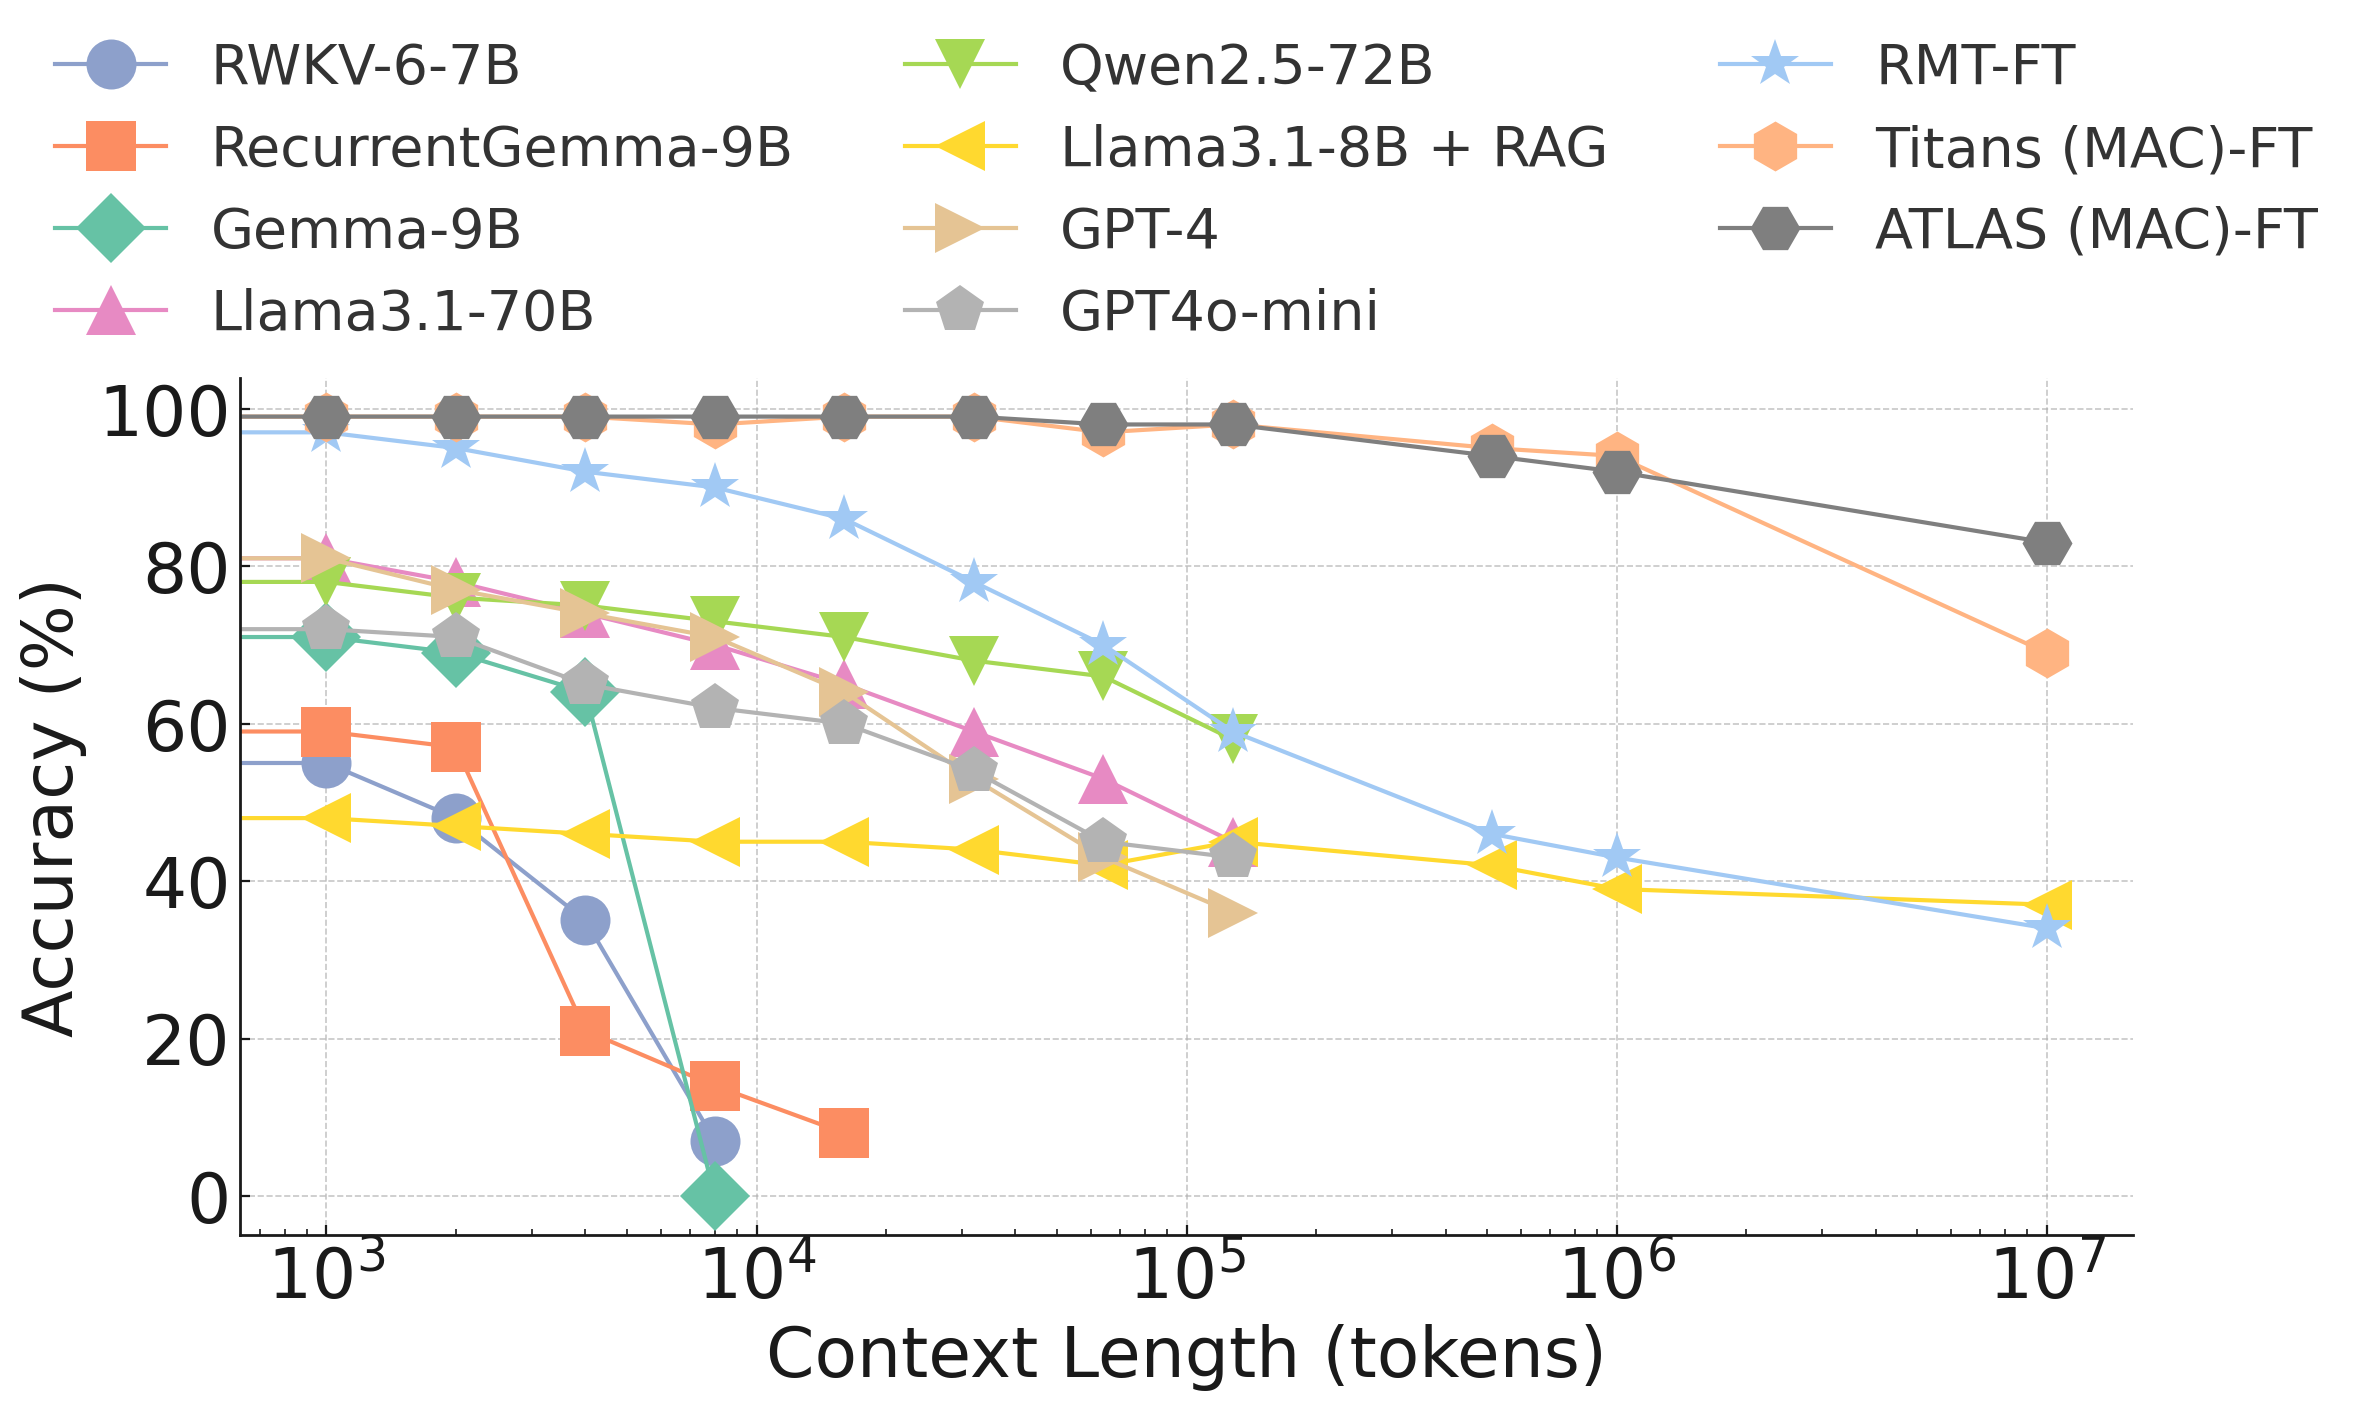
\includegraphics[width=0.8\linewidth]{Images/BABILong.png}
    \captionof{figure}{Performance of \model{} and baselines on BABILong benchmark. \model{} surpasses Titans performance and effectively scale to 10M context length in this task.}
    \label{fig:babilong}
    \end{minipage}~
    \hfill~
    \begin{minipage}[t]{0.49\textwidth}
    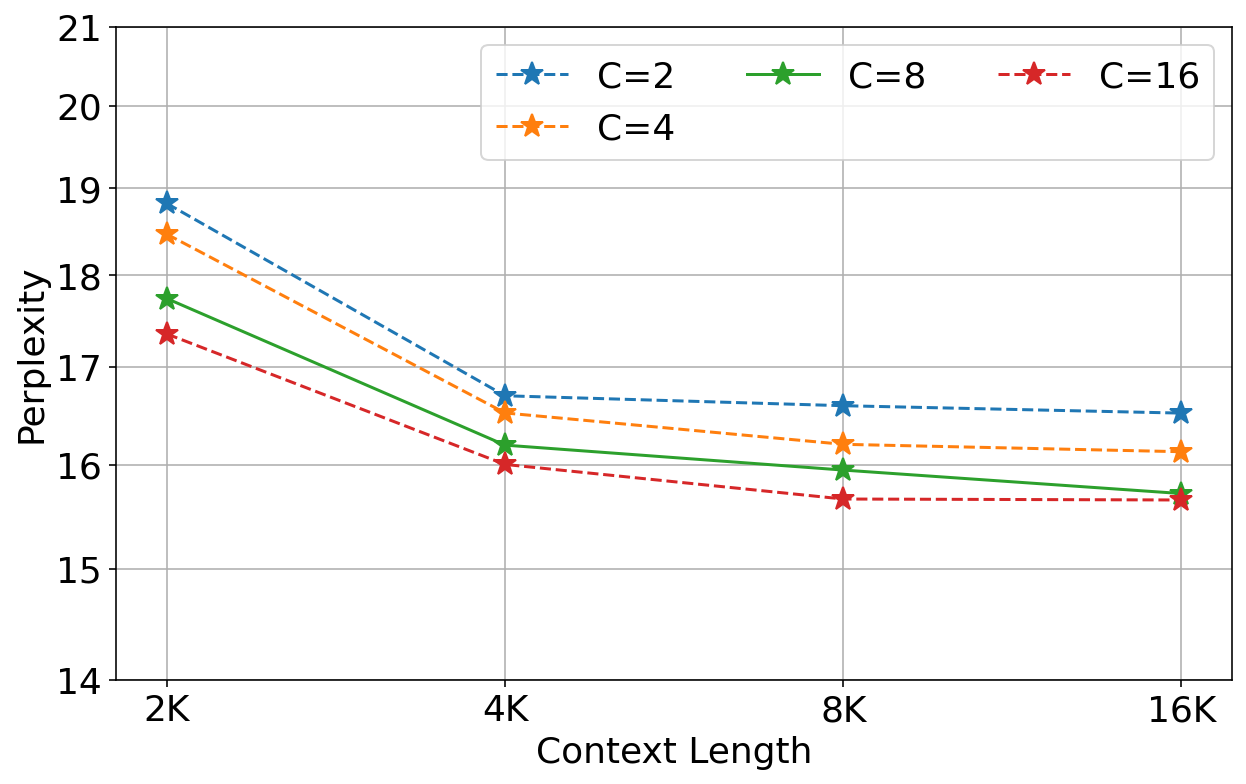
\includegraphics[width=0.8\linewidth]{Images/effect-of-context.png}
    \captionof{figure}{The effect of local context length (i.e. $c$) on the performance of \omodel{} with different global context length.}
    \label{fig:effect-c}
    \end{minipage}
\end{minipage}









\subsection{Long Context: Needle In a Haystack}\label{sec:niah}
One of our main motivations to design \model{} is to enhance the performance of long-term neural memory module in long context tasks. Accordingly, to evaluate the effectiveness of our designs for improving the effective context length and memory capacity, we perform an experiment on needle-in-haystack tasks of RULER~\citep{hsieh2024ruler} benchmark. The performance of \model{} and its hybrid variants, as well as our Transformer-like architectures and baselines are reported in \autoref{tab:hystack}. \model{} shows very good performance compared to the recurrent baselines, outperforming modern recurrent neural networks such as Titans and DeltaNet. Its hybrid variants further improve its effective context length, effectively extrapolating to sequences with $\times 4$ of their training context size. We attribute this performance to the proposed enhancements for the capacity of the memory. We further perform ablation studies to validate this claim. Also, our Transformer-like architectures outperforms the baselines, even our hybrid variants of \model{} in longer contexts. This shows the importance of exponential feature mapping in longer sequences.





\subsection{Long Context: BABILong Benchmark}\label{sec:babilong}
To compare the effectiveness of \model{} with Titans \citep{behrouz2024titans} in ultra-large sequences, we further evaluate \model's performance on BABILong benchmark~\citep{kuratov2024babilong}. In this experiment, we follow \citet{behrouz2024titans} and use MAC architecture but without persistent memory tokens. We also follow the original setup in the benchmark and fine-tune our model. The results are reported in \autoref{fig:babilong}. While \model{} shows competitive and on par performance with Titans until 1M context length, the performance of Titans drops in 10M. \model, however, maintains its performance and achieve +80\% accuracy in 10M context length. We attribute this to more powerful memory; in terms of (1) memory management (i.e., the use of Muon), (2) better memory capacity due to polynomial kernels, and (3) its nature to memorize the context, instead of individual tokens. 





In previous sections, we show the effectiveness of our Transformer-like architectures (i.e., \textsc{DeepTransformer}s and \textsc{Dot}) in both language modeling and long-context needle-in-haystack tasks. From now on, we focus on our recurrent architectures (i.e., \model, and \omodel) to show the importance of presented improvements. 




\subsection{Learnability Experiments}
We have also performed some small-scale experiments to analyze the function-learning capability of small MLPs in an online fashion. In this setting, we have a sequence of tuples $(i_1, o_1), \ldots (i_t, o_t)$ with both $i_j, o_j \in \mathbb{R}^d$ for all $j$. We train an MLP $\mathcal{M}$ in an online fashion to minimize $\text{loss}_j = \|{i_j - o_j}\|_2^2 / \|{o_j}\|_2^2$ -- specifically, we compute the gradient at time step $j$ as $\nabla_{\mathcal{M}\text{.params}} \text{loss}_j$  and use standard optimizers such as Adam, Rmsprop and SGD to update the parameters. Such experiments help us understand the representation power of the models we use to represent memory and the power of optimization algorithms to quickly learn the underlying sequence mapping.











\begin{figure*}
  \begin{center}
  \begin{subfigure}[t]{.39\textwidth}
    \centering
    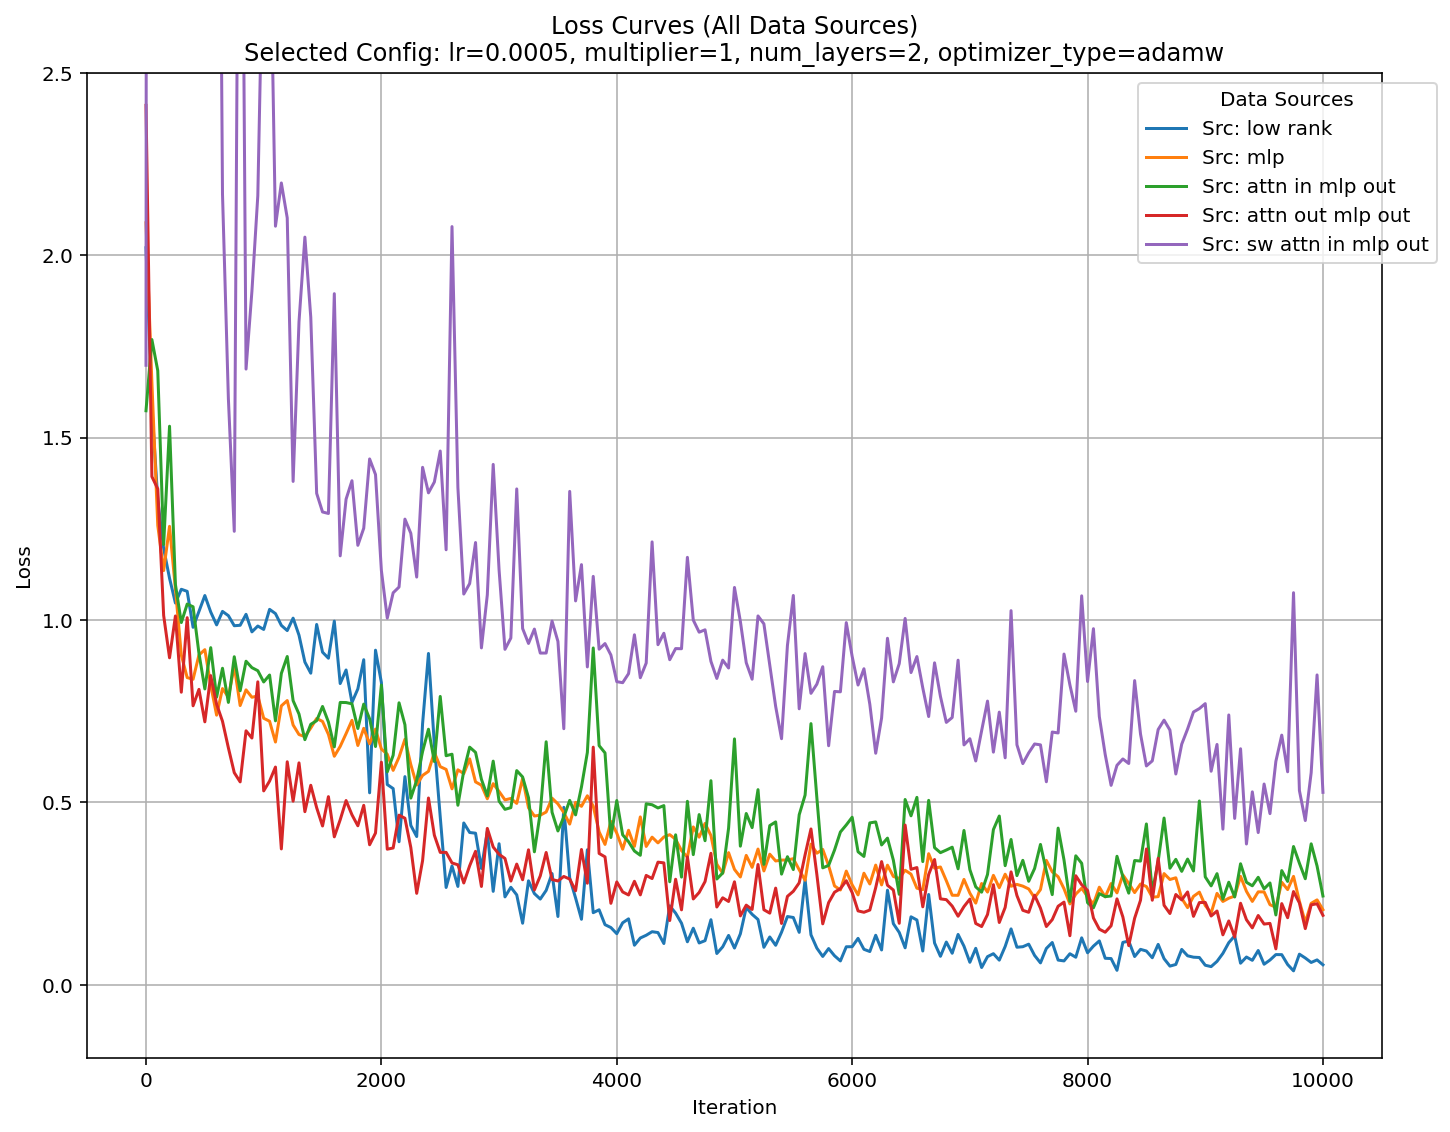
\includegraphics[width=\linewidth]{Images/download_multiplier_1_num_layer_2_adamw_lr_p0005.png}
    \caption{$\mathcal{M}$ with 2 hidden layers and no expansion.}
  \end{subfigure}
    \hspace{3ex}
  \begin{subfigure}[t]{.39\textwidth}
    \centering
    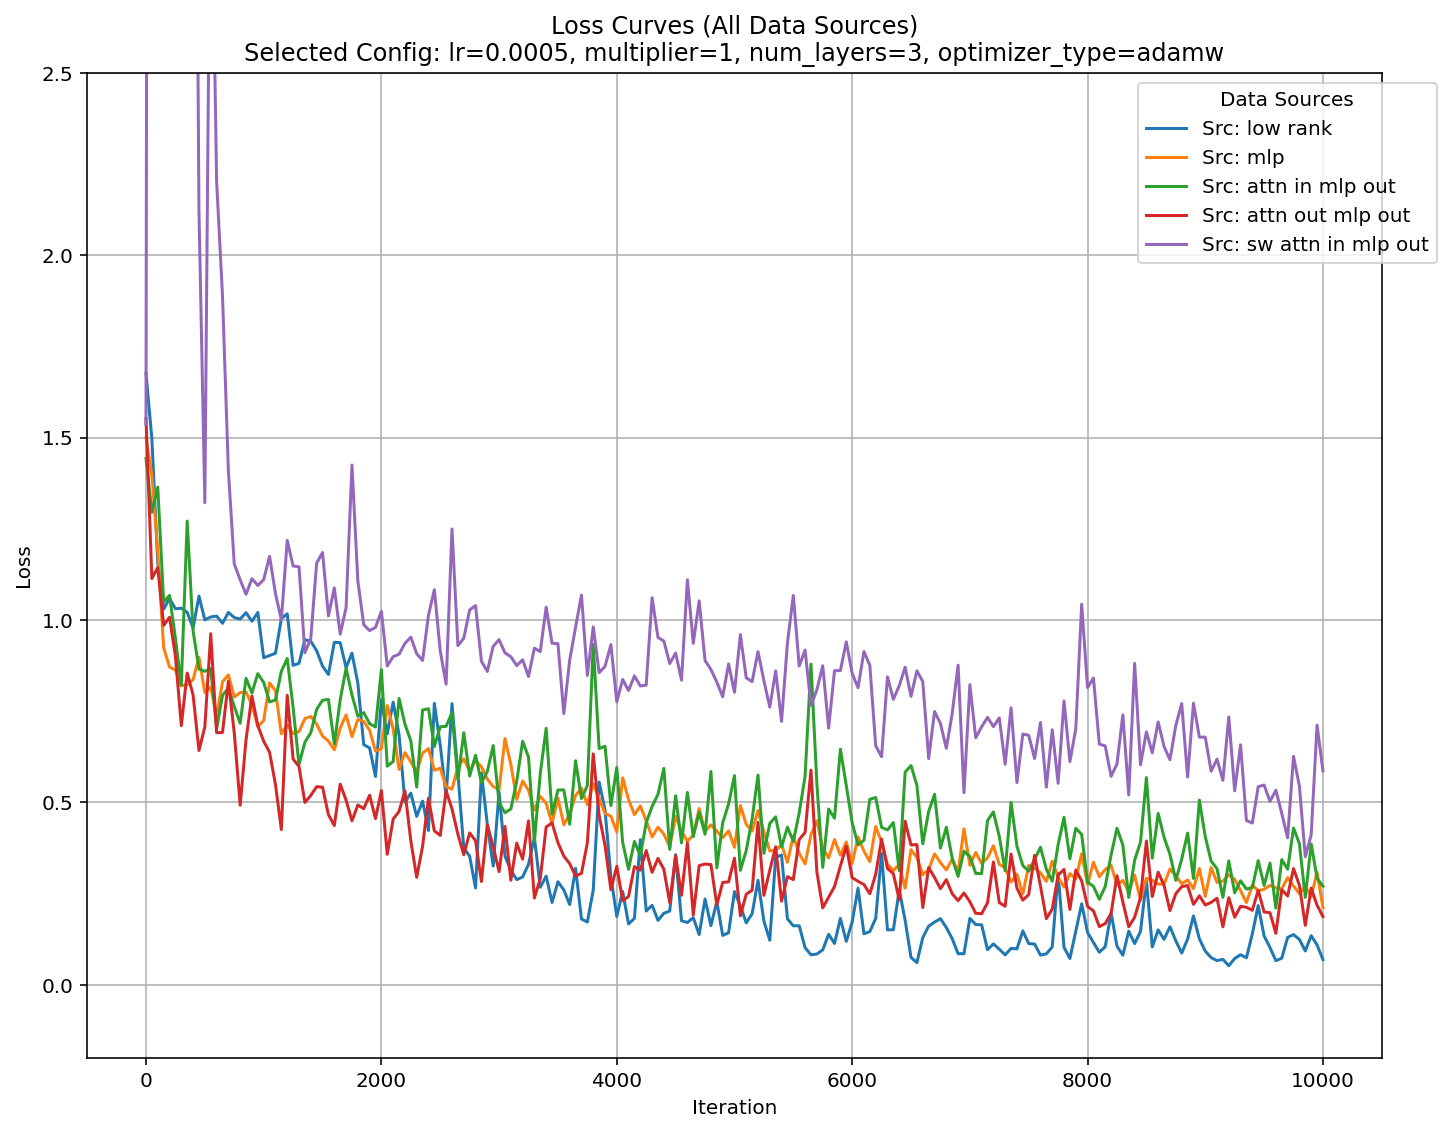
\includegraphics[width=\linewidth]{Images/download_multiplier_1_num_layer_3_adamw_lr_p0005.png}
    \caption{$\mathcal{M}$ with 3 hidden layers and no expansion.}
  \end{subfigure}
  \medskip
  \begin{subfigure}[t]{.39\textwidth}
    \centering
    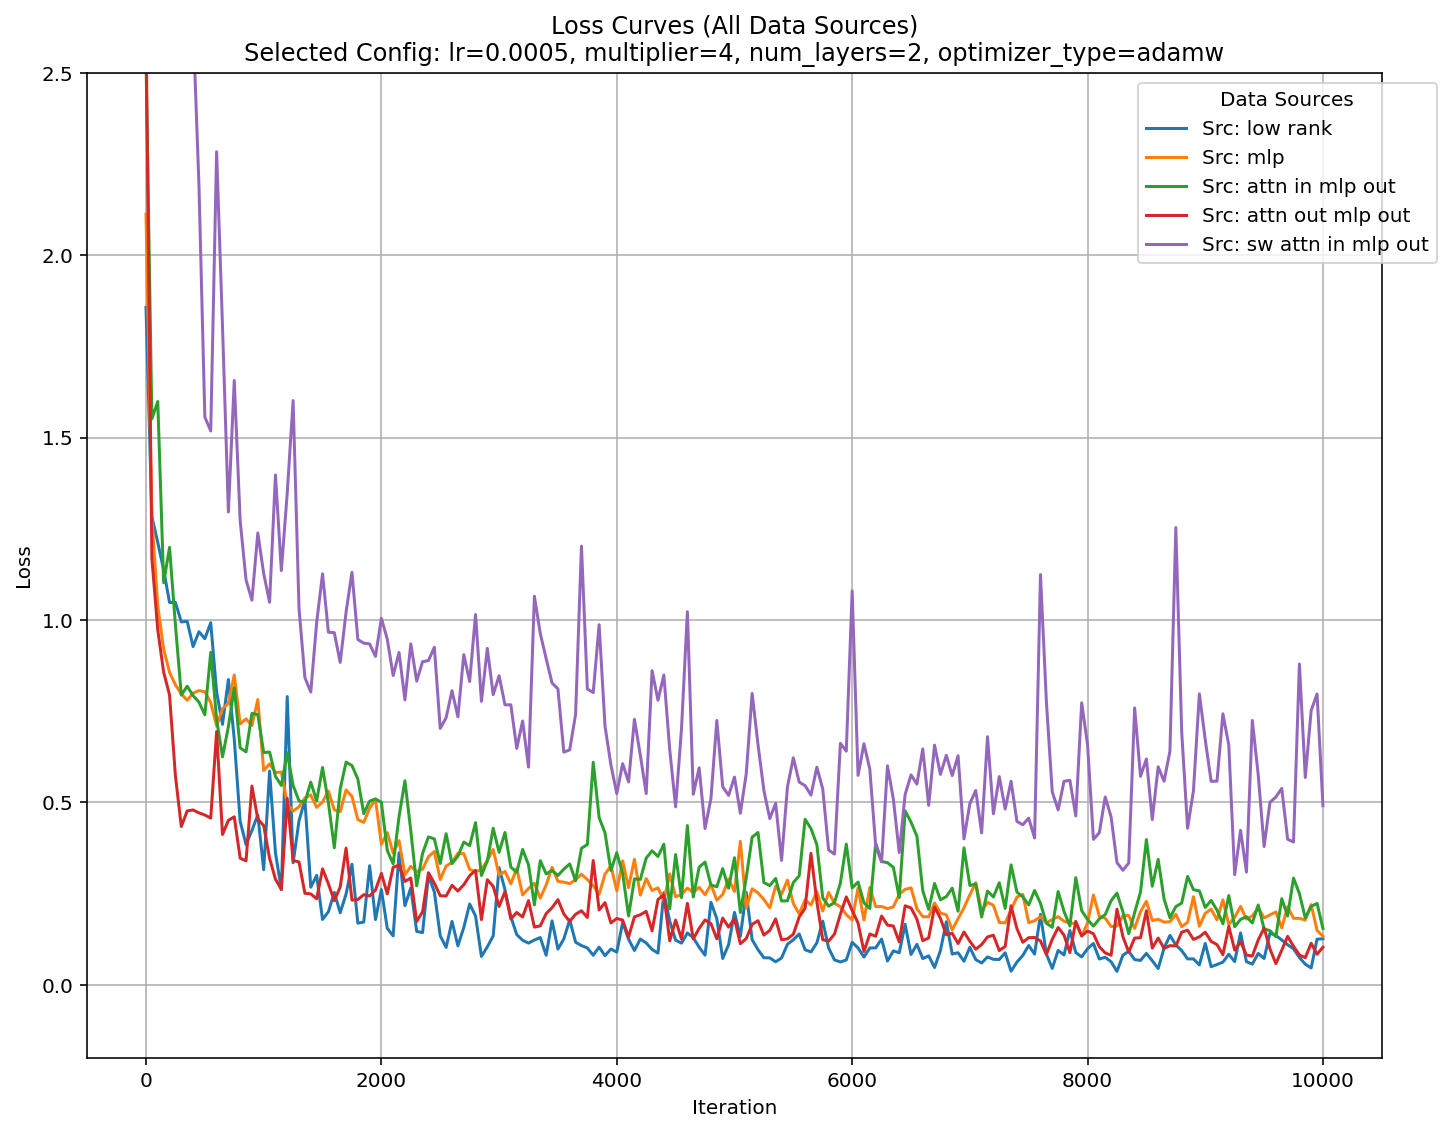
\includegraphics[width=\linewidth]{Images/download_multiplier_4_num_layers_2_adamw_lr_p0005.png}
    \caption{$\mathcal{M}$ with 2 hidden layers and 4x expansion.}
  \end{subfigure}
  \hspace{3ex}
  \begin{subfigure}[t]{.39\textwidth}
    \centering
    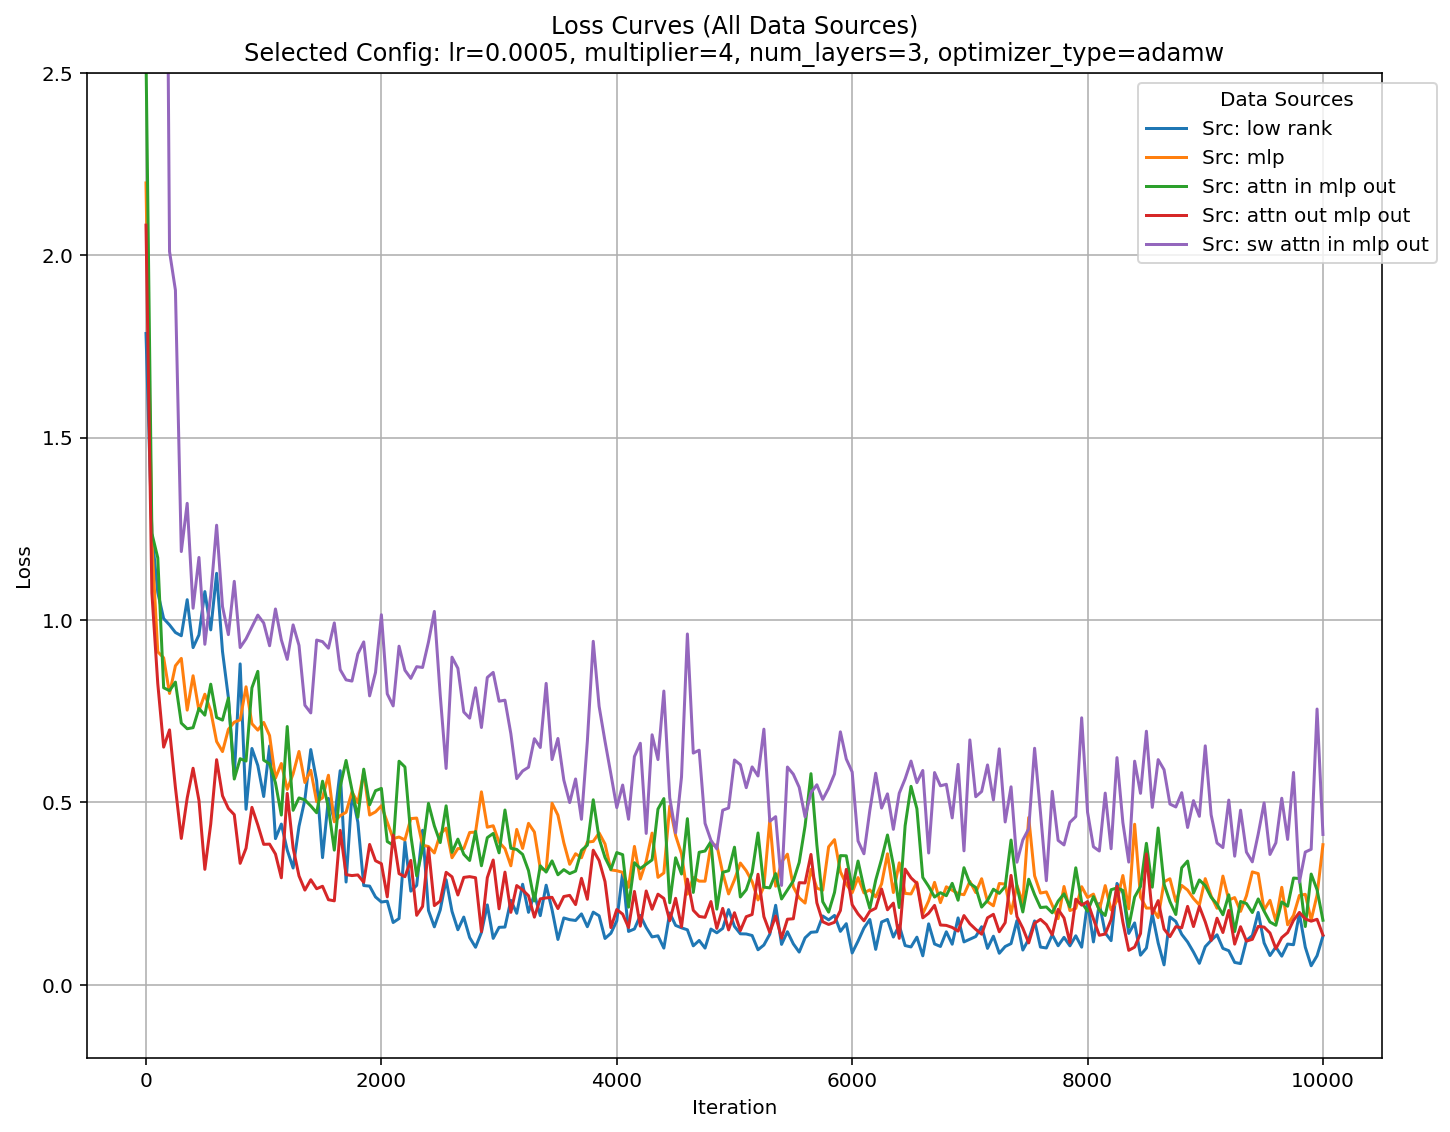
\includegraphics[width=\linewidth]{Images/download_multiplier_4_num_layers_3_adamw_p0005.png}
    \caption{$\mathcal{M}$ with 3 hidden layers and 4x expansion.}
  \end{subfigure}
  \vspace{-2ex}
  \caption{Loss curves for different setting with various hyperparameters}
  \label{fig:learnability-1}
  \end{center}
\end{figure*}





We study five different sequence to sequence functions:
\begin{enumerate}
    \item \textbf{Low Rank Mappings}: We sample a random low rank matrix $\mathbf{W} = \mathbf{X}\mathbf{Y}$ with $\mathbf{X} \in \mathbb{R}^{d \times k}$ and $\mathbf{Y} \in \mathbb{R}^{k \times d}$. We then sample $i_1, \ldots, i_t$ randomly from a Gaussian distribution and set $o_j = \mathbf{W}^{\mathsf{T}} \cdot i_j$ for all $j \in [t]$.
    \item \textbf{MLP Mappings}: We sample an MLP $\mathcal{M}$ with 1 input, 1 hidden and 1 output layer which uses GELU non-linearity. We set the hidden dimension to $d$ so that there is no expansion. We then sample $i_1, \ldots, i_t$ randomly from a Gaussian distribution and then set $o_j = \mathcal{M}(i_j)$ for all $j \in [t]$.
    \item \textbf{Attention+MLP Mapping}: We sample $(i_1, \ldots, i_t)$ from a Gaussian distribution and an MLP $\mathcal{M}$ as above. We additionally sample three $d \times d$ matrices $\mathbf{W_Q}$, $\mathbf{W_K}$ and $\mathbf{W_V}$ and compute $q_j = \mathbf{W_Q}^{\mathsf{T}} \cdot i_j$, $k_j = \mathbf{W_K}^{\mathsf{T}} \cdot i_j$ and $v_j = \mathbf{W_K}^{\mathsf{T}} \cdot i_j$ for all $j \in [t]$. We then compute $o'_1, \ldots, o'_t$ as outputs of the causal masked attention mechanism applied on $\{q_j\}_{j \in [t]}, \{k_j\}_{j \in [t]}, \{v_j\}_{j \in [t]}$ and finally compute $o_j = \mathcal{M}(o_j)$.
    \item \textbf{Attention Outputs as Inputs}: We do the same as above except that we output $o'_j$ as the input sequence and $o_j$ as the output sequence.
    \item \textbf{Sliding Window Attention + MLP Mapping}: We do the same as in \textbf{Attention + MLP Mapping} setting except that we use a sliding window attention instead of full attention. We use a sliding window of 512 in our experiments.
\end{enumerate}
Note that the settings 3 and 5 are much harder to learn since they require (partially) memorizing the previous inputs and outputs to be able to learn the function that maps $i_j$ to $o_j$, whereas the settings 1, 2 and 4 do not need to memorize the previous input-output pairs and just need to learn the underlying low-rank matrix or the MLP that maps the inputs to outputs.

The setting 4 is slightly different to setting 2 in that the inputs are not-independent at each time step and are correlated by the attention mechanism we use to compute the inputs. Thus a strong learning algorithm maybe able to utilize the underlying correlations to learn the mapping faster in setting 4 versus setting 2. 





\begin{table*}
    \centering
    \caption{Performance of \model, \omodel, and baselines on the synthetic benchmark of MAD~\citep{poli2024mechanistic}. \model{} outperforms all the baselines, including Transformers.}
    \label{tab:MAD}
    \resizebox{0.8\linewidth}{!}{
    \begin{tabular}{l c c c c c c}
    \toprule
         &  \multirow{2}{*}{Compression} & \multirow{2}{*}{(Noisy) ICR} & \multirow{2}{*}{Fuzzy ICR} & Selective & \multirow{2}{*}{Memorization}  & \multirow{2}{*}{Average}\\
         &  & & & Copying & \\
         \midrule
         \midrule
        Transformers & 49.4 & 100 & 48.2 & 95.9 & 83.8 & 75.46\\
         Gated DeltaNet & 44.8 & 100 & 32.5 & 96.2 & 81.7 & 71.04\\
         Titans & 49.6 & 100 & 49.7 & 99.4 & 83.5 & 76.44\\
         \midrule
         \omodel{} (ours) & 50.9 & 100 & 54.2 & \cellcolor{myblue} 99.6 & 90.2 & 78.98\\
         \model{} (ours) & \cellcolor{myblue}51.6 & \cellcolor{myblue} 100 &  \cellcolor{myblue} 54.9 & \cellcolor{myblue} 99.6 & \cellcolor{myblue} 91.4 & \cellcolor{myblue}79.50\\
    \toprule
    \end{tabular}
    }
\end{table*}



\begin{minipage}[t!]{\textwidth}
  \begin{minipage}[t]{0.60\textwidth}
    \centering
    \captionof{table}{The performance of our models (\model, and \omodel) compared to baselines. While still Transformers achieve the best results in in-context recall tasks, our design of context memorization and polynomial feature maps can close the gap with Transformers. }
    \label{tab:recal}
    \resizebox{\linewidth}{!}{
    \begin{tabular}{l c c c c c c c}
    \toprule
         &  \multirow{1}{*}{SWDE} & \multirow{1}{*}{NQ} & \multirow{1}{*}{DROP} & FDA & SQUAD & \multirow{1}{*}{TQA} & Average \\
         \midrule
         \midrule
        Transformers & \cellcolor{myblue}84.9 & \cellcolor{myblue}23.0 & \cellcolor{myblue}28.4 & \cellcolor{myblue}72.5 & \cellcolor{myblue}48.1 & \cellcolor{myblue}64.4 & \cellcolor{myblue} 53.55\\
         Gated DeltaNet & 63.2 & 19.1 & 26.7 & 33.4 & 39.6 & 59.7 & 40.28\\
         Titans & 65.1 & 20.7 & 27.2 & 37.3 &  42.6 & 61.0 & 42.31\\
         \midrule
         \omodel{} (ours) & \underline{67.4} & 21.1  &  27.2  & 39.0 & 43.2 & 60.9 & 43.13\\
         \model{} (ours) & 66.8  & \underline{21.9}  &  \underline{27.4}  & \underline{40.7} & \underline{44.1} & \underline{61.3} & \underline{43.70}\\
    \toprule
    \end{tabular}
    }
  \end{minipage}~\
  \hfill~
  \begin{minipage}[t]{0.40\textwidth}
    \centering
    \captionof{table}{Ablation Study on \model. All components of \model{} are positively contributing to its performance. }
    \label{tab:ablation}
    \resizebox{\linewidth}{!}{
    \begin{tabular}{l c c}
    \toprule
    \multirow{2}{*}{Model}     & Language Modeling & C.S. Reasoning \\
    & ppl $\downarrow$ & acc $\uparrow$ \\
    \midrule
    \midrule
    \model{}         &   19.97  &  52.77  \\ 
    \midrule
    \hspace{6pt}+{Gated MLP Memory} & 19.53 & 53.09                \\
    \midrule
    \hspace{6pt}+\texttt{Attn} (MAG) & 19.90 & 53.08                \\
    \hspace{6pt}+\texttt{Attn} (MAL) & 20.26 & 52.63               \\
    \midrule
    Linear Memory          & 21.03   &  49.74    \\
    w/o Muon      & 19.65   &  52.56    \\
    $c = 1$                & 21.98   &  49.26    \\
    w/o Polynomial Mapping  &  22.14   &  50.57   \\
    \toprule
    \end{tabular}
    }
  \end{minipage}
\end{minipage}



We set $d = 256$ and show the loss curves vs sequence position for all the five settings with function learning MLP $\mathcal{M}$ being defined and trained with different settings in Figure~\ref{fig:learnability-1}. We can see that in all the settings, the model learns non-trivial mappings from inputs to outputs with the $loss_j = \|i_j - o_j\|_2^2/\|o_j\|_2^2$ being smaller than $1$ eventually. Most notably, the correlations in inputs in setting 4 induced by the attention mechanism makes the model quickly learn the mapping compared to in setting 2 and the models usually learn the best in setting 1 which is the least complex function.  

The models do the worst in settings 3 and 5 which require the models to (partially) memorize the inputs and outputs to learn the attention mechanism outputs. Surprisingly, the models learn to do better in setting 3 vs setting 5, when we would expect that capacity requirement for setting 3 to be higher than setting 5. We hypothesize that the learning algorithm is unable to make the model `forget' old inputs which makes the loss worse in sliding window setting when compared to global attention setting. A caveat of our analysis is that, the attention computation is done on randomly initialized vectors and hence the attention matrix is usually not spiky, unlike in the attention matrix for trained set of query, key and value vectors in LLMs. This leads to attention outputs being close to the mean of value vectors in the context.























\subsection{Additional Experiments: In-context Recall, MAD Synthetic Benchmark, and Associative Recall}\label{sec:retrieval-tasks}
In this section, we first evaluate the performance of our models on MAD benchmark, a synthetic benchmark that evaluate the performance of models in recall, memorization, compression, and copying tasks~\citep{poli2024mechanistic}. The results are reported in \autoref{tab:MAD}. \model{} achieves the best results in all aspects, particularly in memorization, which shows the importance of its components for enhancing the memory capacity. 


In-context recall tasks is one of the most challenging benchmarks for recurrent neural networks. In this section, we follow \citet{arora2024simple} and perform experiments on SWDE~\citep{lockard2019openceres}, NQ~\citep{kwiatkowski2019natural}, DROP~\citep{dua2019drop}, FDA~\citep{arora2023language}, SQUAD~\citep{rajpurkar2016squad}, and TQA~\citep{kembhavi2017you} to evaluate and compare the performance of \model{} with baselines and Transformers. The results are reported in \autoref{tab:recal}. While Transformers still achieve the best results in in-context recall tasks, \model{} and \omodel{} shows competitive performance and performs better than state-of-the-art recurrent models. We again attribute this performance to better memory management and capacity.



\begin{minipage}[t!]{\textwidth}
    \begin{minipage}[t]{0.33\textwidth}
    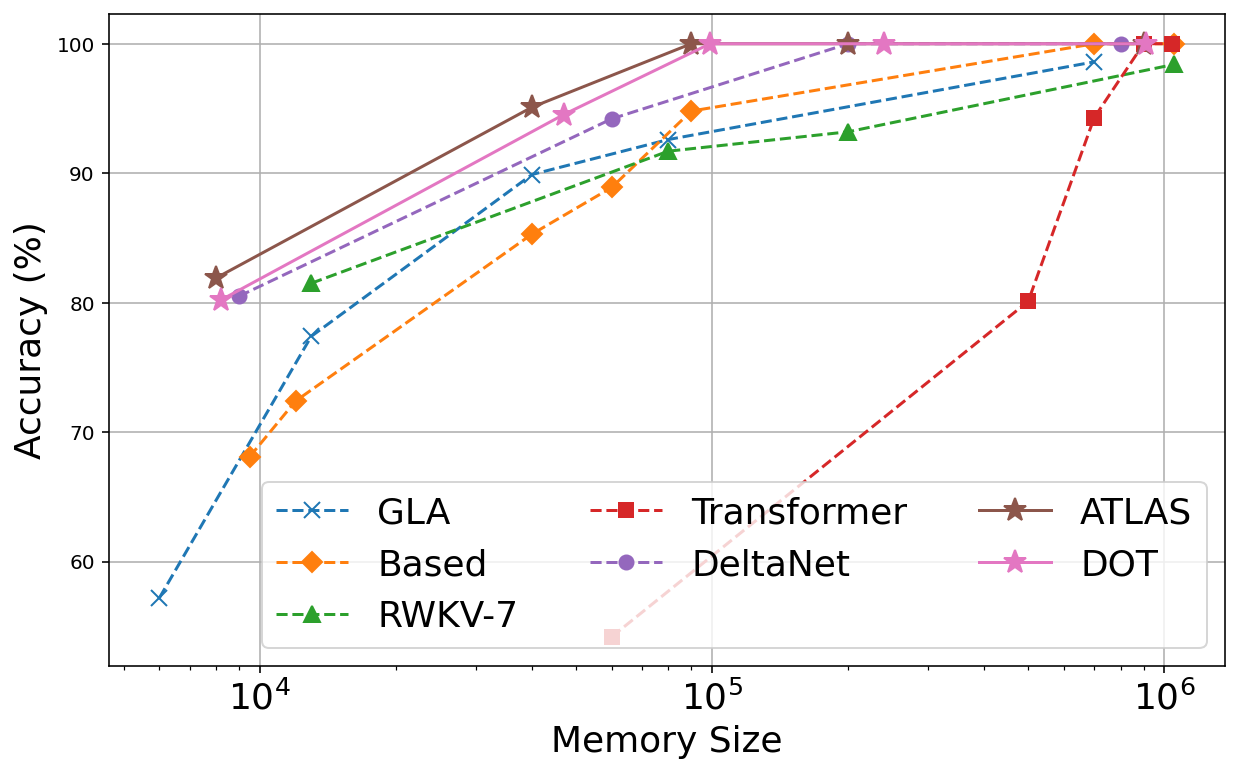
\includegraphics[width=\linewidth]{Images/MQAR-results.png}
    \captionof{figure}{The results for associative memory recall.}
    \label{fig:AMR}
    \end{minipage}~
    \hfill~
      \begin{minipage}[t]{0.66\textwidth}
    \centering
    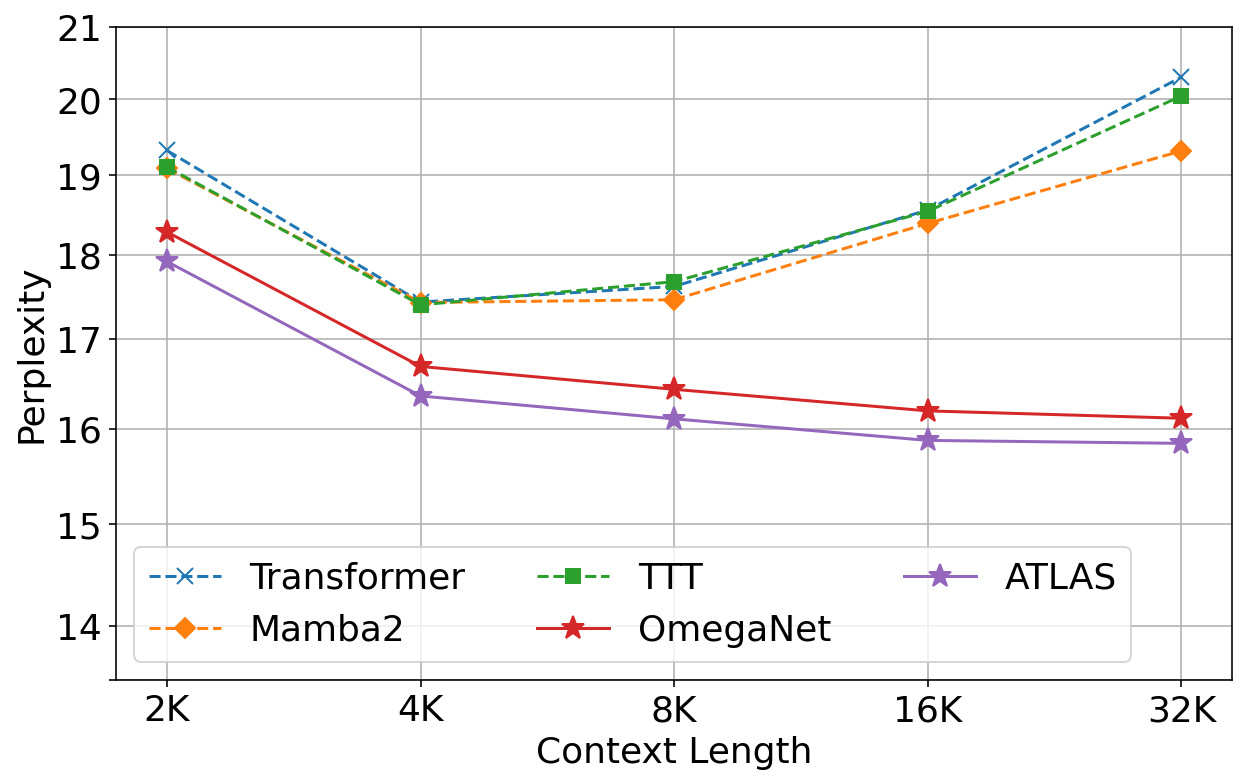
\includegraphics[width=0.5\linewidth]{Images/context_length_ATLAS.png}~
    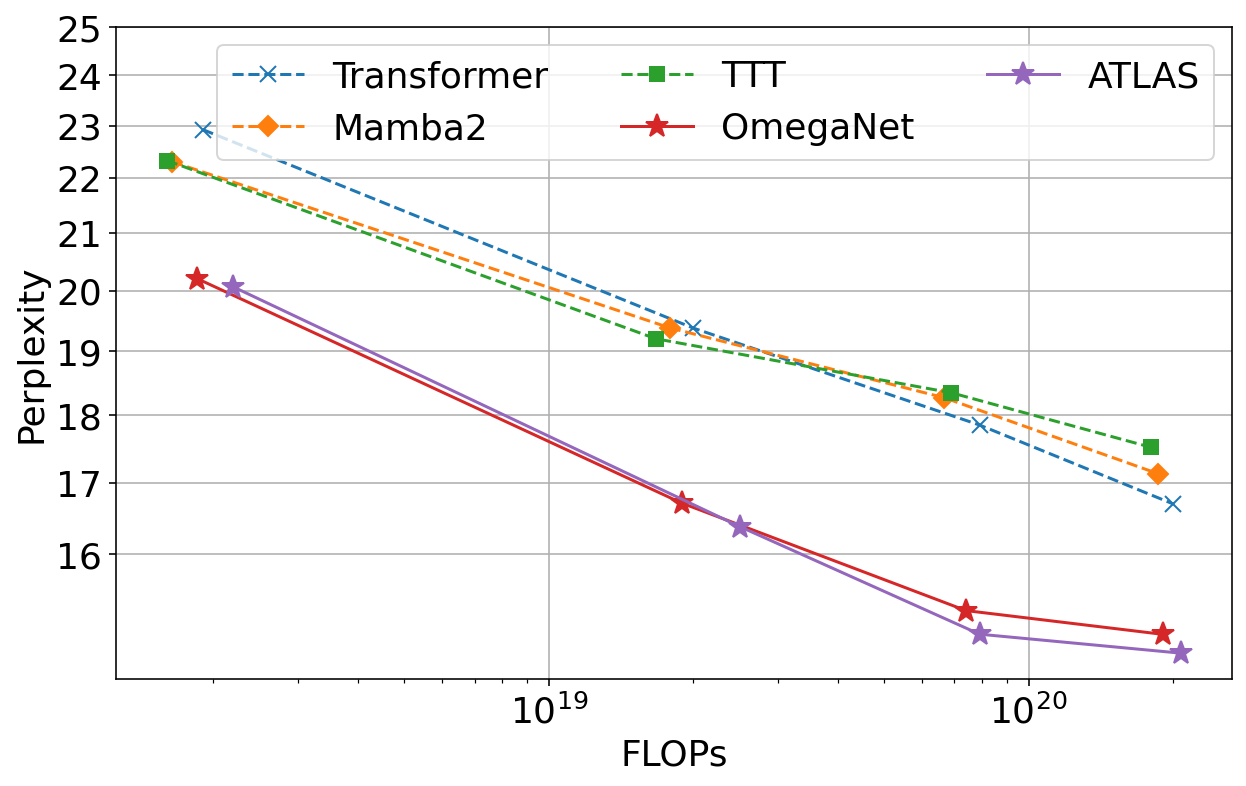
\includegraphics[width=0.5\linewidth]{Images/Model_Size_ATLAS.png}
    \captionof{figure}{Scaling patterns of \model, and \omodel{} with respect to (Left) training context length, and (Right) FLOPs. }
    \label{fig:scaling}
    \end{minipage}
\end{minipage}

Finally, following \citet{yang2024parallelizing} and \citet{arora2023zoology} we evaluate the performance of \model{} and \textsc{Dot} in Multi-Query Associative Recall (MQAR) task~\citep{arora2023zoology}. The results are reported in \autoref{fig:AMR}. Both models show good performance compared to baselines and \model{} achieve the best performance per memory size compared to state-of-the-art models such as DeltaNet~\citep{yang2024parallelizing}. 








\subsection{Ablation Study and Scaling Patterns}
In this section, we perform an ablation study on the differernt components of \model, and also evaluate its scaling patterns with respect to the number of parameters and also the context length of the training. The results for ablation study are reported in \autoref{tab:ablation}. The results show that: (1) more powerful memory architectures such as gated MLP can further enhance the performance of \model; (2) The hybrid variants further improve the performance, where MAG shows better improvement compared to MAL architecture; (3) Polynomial mappings as well as deep memory are particularly important when we use context memorization (i.e., \learningrule{} rule). \autoref{fig:effect-c} also shows the effect of local context length (i.e., $c$) on the performance of the model. With the increase of $c$ we can achieve better performance, mainly due to the gating parameters of $\gamma$ that can prune the context, whenever it is needed. 





\head{Model Size}
\autoref{fig:scaling} shows the scaling pattern of \model, and \omodel, with respect to number of parameters and compared to baseline. Both models achieve a good scaling pattern with increasing the model size, achieving lower perplexity in all scales compared to baselines. 




\head{Context Length}
\autoref{fig:scaling} shows the scaling pattern of \model, and \omodel, with respect to the context length and compared to baseline. Both models due to high memory capacity can scale well, when increasing the context length. 


